\documentclass[a4paper,11pt,hidelinks]{article}

%%%%%%%%%
%%usees%%
%%%%%%%%%
\usepackage[utf8]{inputenc}
%\usepackage[ngerman]{babel}
%\usepackage{a4wide}
\usepackage[margin=3.0cm, top=3.0cm, bottom=3.0cm]{geometry}
\usepackage{setspace}
\usepackage{graphicx}
\usepackage{amssymb} 
\usepackage{amsmath}
\usepackage{mathtools}
\usepackage{footnote}
\usepackage{caption}
\usepackage{color}
\usepackage[hidelinks]{hyperref}
\usepackage{cite}



%%%%%%%%%
%%Title%%
%%%%%%%%%

\author{Frederik Zwilling 304314}
\title{Bachelor-Thesis Proposal:\\ Simulation of the RoboCup Logistic League with Fawkes and Gazebo for Multi-Robot Coordination Evaluation}
\begin{document}
%\thispagestyle{empty}
%\tableofcontents
%\newpage
%\onehalfspace
\maketitle
%%%%%%%%%
%%Text%%
%%%%%%%%

\section{Introduction}
Autonomous multi-robot systems are about to play an important role in the future of logistics and production. They are able to save time and cost in logistics and the industrial production process. Existing systems in the warehousing domain, such as~\cite{{Kiva}}, already show the potential of autonomous robots to boost efficiency in many ways. Multi-robot-systems have a big potential because they are able to do work distributed and in parallel. On the one hand parallelism is challenging and complex. On the other hand, multiple robots working in parallel can solve tasks, such as warehousing, more efficiently than single robots. Though, the development of multi-robot systems for logistics can be difficult because the robots have to handle many complex tasks. They have to detect objects, localize themselves, make a plan of what to do in which order, coordinate with other robots, optimize the work flow and be safe for humans and hardware at all times.\\
A key to effective and time saving development of reliable software for robots is simulation. Simulation makes it possible to test and compare different approaches quickly. This leads to a better quality of the software and better performance of the robot. By simulating the behavior of a multi-robot system much time can be saved because there are no real robot which have to be set up and the simulation can quickly change between different scenarios. Simulation also enables testing if no real robots are available and can be easily used to compare different versions of the software. For example this can be useful to find unknown parameters such as thresholds.\\
The proposed bachelor-thesis will develop a multi-robot simulation environment for the \textit{Logistic League Sponsored by Festo} (LLSF) and the robot software framework \textit{Fawkes}\footnote{\url{http://www.fawkesrobotics.org}}. To tackle the goal of a multi-robot simulation, a basis simulation, that is able to properly simulate single robots, is needed. If this basis simulation works on a high level to provide ground truth and a low level to provide sensor data as well, most of the problems in the development of the robot system can be simulated. As a basis simulation, the Open Source simulator \textit{Gazebo} was chosen.\\
In the following the proposal shows the background of the thesis in section 2. Section 3 gives an overview of related work. Other simulators and multi-robot simulations are analyzed there. Furthermore the section describes the current multi-agent strategy and the auction-based method Murdoch. Section 4 presents the proposed work in detail. It defines goals, gives a schedule and discusses how the evaluation of the thesis will be done. The conclusion is found in section 5.


\section{Background}
\subsection{Logistic League Sponsored by Festo}
The Logistic League Sponsored by Festo (LLSF) is part of \textit{RoboCup}, an international robotics competition founded in 1997. The RoboCup provides standard problems as a platform for artificial intelligence and robotics research~\cite{{Robocup}}. There are different leagues in the RoboCup. The main focus is on soccer leagues, but there are more leagues, such as the leagues for rescue, domestic and logistic robots. LLSF is one of those leagues. LLSF aims to foster scientific work on autonomous solutions for logistics and to provide a testbed for existing approaches~\cite{LLSFTestbed}. The participants should find new approaches and improve already existing ones to optimize material and information flow in logistics. LLSF takes place  in a simplified production hall~\cite{LLSFRules}. 
\begin{figure}
\centering
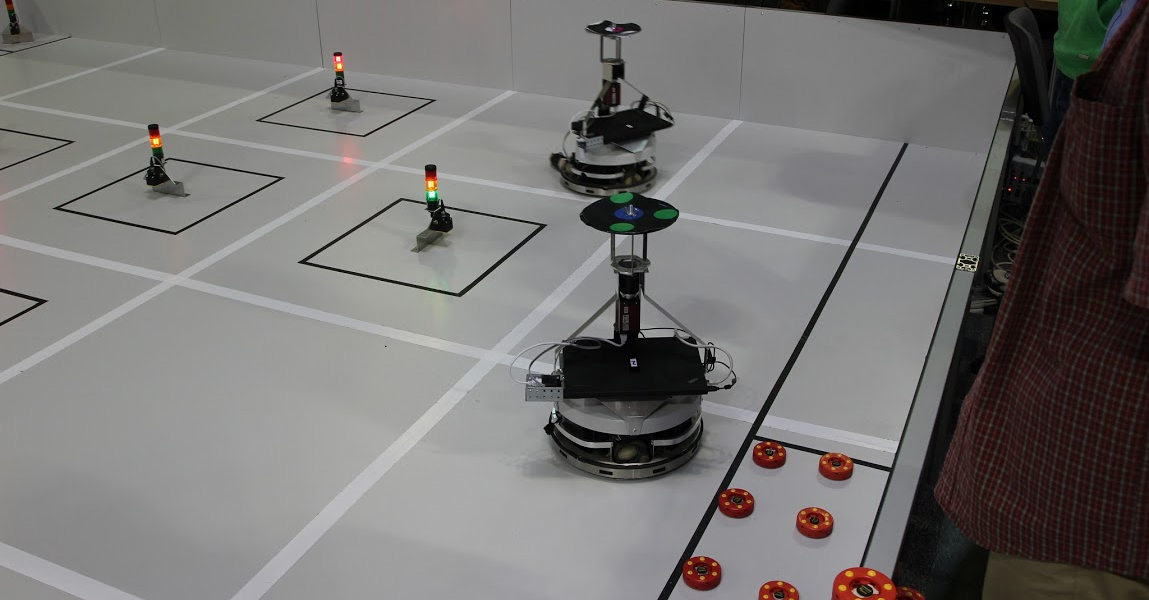
\includegraphics[scale=0.3]{pics/llsf}
\label{Figure 1}
\caption{A half of the LLSF field. Two Robotinos of the Carologistics team at the RoboCup German Open 2013}
\end{figure}
Figure 1 shows a part of the 5.6m x 5.6m hall with two Carologistic robots, three machines and some material-pucks. The main task of LLSF is to produce and deliver ordered products as efficient as possible by feeding machines with resources and semi-finished products. The participants can use up to three Robotino robots by Festo~\cite{{Robotino}}. They hold omni-directional wheels, a gripper to move pucks, and other sensors added by the participants. The orange pucks represent resources and products. They are equipped with an RFID-chip\footnote{Radio-frequency identification allows the wireless identification of objects with small chips.} which is needed to store the different product states of the pucks. The light-signals on top of the RFID-readers represent the machines. They convert resources or semi-finished products into products and trash. There are different types of machines. They can produce different product-types, produce intermediate products, recycle trash or are used for the delivery of products. The light-signals on top of the machines indicate the machine-status. Beside these visual elements, there is also a referee box (refbox), which controls the machines and communicates with the robots during the game. The refbox gives orders which products are to be produced, informs the robots about the game state and rewards points for achieved goals.
\subsection{Fawkes}
\sloppy
Fawkes is an Open Source robot software framework developed primarily at the Knowledge-based Systems Group\footnote{\url{http://www.kbsg.rwth-aachen.de/}} at RWTH Aachen University. It is written for Unix systems and follows a component-based software design~\cite{{FawkesDesign}}. It provides an infrastructure to load and unload binary components (implemented as plugins) at run-time and provides a blackboard for communication between the plugins. A plugin can access the blackboard via interfaces. Furthermore it organizes the plugin activity in threads to make use of multi-core architectures. Because of this design, Fawkes is flexible and dynamic. The interchangeability of the plugins, which is caused by the well defined interfaces, makes hardware abstraction and reuse easy. This is also an important advantage for the development of the simulation because the simulation can easily exchange the lower-level robot control and sense plugins. The robot control plugins on higher levels can operate as usual because the interface is the same.\\
Fawkes is comparable to the Robot Operating System ROS~\cite{{Ros}}. ROS is an Open Source framework designed to operate on many robot platforms and to provide a standardized integration framework. It provides a collection of  useful libraries and tools for the development process of robot-software. ROS is widely used and has a large community. In comparison to ROS, the advantage of Fawkes is the tighter integration of the used components. The main loop of Fawkes controls the execution order of all component threads. This makes it possible to match certain time criteria for the components and to provide a \textit{sense-think-act} cycle.
\subsection{Gazebo}
Gazebo is an Open Source robot simulator~\cite{{GazeboDesign}}. It provides a platform to simulate the behavior of robots and other objects physically in a three dimensional world. The Open Source engine Ogre\footnote{\url{http://www.ogre3d.org}} is used for the graphical presentation of the simulation and allows realistic graphical environment. This is important for the simulation of camera sensors. Physics are simulated with the Open Dynamics Engine\footnote{\url{http://www.ode.org}}. Gazebo was originally developed for outdoor applications and aims to simulate robots in a complex and realistic environment. Besides the physical simulation, it does this by generating data for different types of sensors. Gazebo can simulate laser range finders, cameras, sonar sensors, bumpers and more. This enables a more realistic simulation. A simulation in Gazebo is developed by creating robot and world models and developing Gazebo-plugins for behavior. These plugins can control objects in Gazebo and communicate with other software.\\
Why Gazebo was chosen as the most suitable simulator for this thesis, is shown in the section about related work.
\subsection{High-Level Agent Design}
The current implementation of the high-level agent of the Carologistics team uses the CLIPS rules engine\footnote{\url{http://clipsrules.sourceforge.net}}. CLIPS is a production system with rule-based, object-oriented and procedural programming paradigms. It uses forward chaining inference, can use functions and can be integrated into C and Java. This integration makes it easy to use CLIPS as a subsystem in other software systems. The CLIPS rules engine was chosen with the intention to use incremental reasoning. This means that the robot can take the next best action at any point in time. With this approach no re-planning is needed as with classical planners. Another cause for this choice was the ability to cope with incomplete knowledge about the world, required in the LLSF scenario~\cite{{Incremental}}. This was due to the rules of 2012. In that year the robots had to deal with incomplete knowledge. They had to figure out the machine-types by trying to feed them with available pucks and looking for the response. By the rules of 2013, the refbox provides the robots with the ground truth about the machine-types. Another change since 2013 is that the Carologistic Robotinos can use a mounted laptop for computing. In 2012 only one of up to three Carologistic Robotinos operated in the competition. All these points show that the multi robot coordination and planning is a necessary step to go further in LLSF.
\subsection{Multi-Robot Coordination}
At the RoboCup 2012 in Mexico, the Carologistic team used a single Robotino in the LLSF competition. Therefore, no multi-robot coordination was necessary. At the RoboCup 2013 in Eindhoven the team used two robots with fixed roles. These roles determine the tasks of the robots over the whole game. One Robotino is assigned to produce the simplest product, which can be produced at a single machine with only one resource puck, and the other one is assigned to produce complex products, for which multiple machines and intermediate products are necessary. Here again, no real coordination strategy is needed. It is only necessary to lock the two positions on the field, that both robots need. These two positions are the input storage, where the robots get new resources and the delivery zone, where the robots deliver finished products. The machines the robots use are disjoint. This task allocation depending on roles is simple to implement and robust against network failure. However, it is neither flexible regarding robot failure nor efficient because the robots can not work on other tasks while the product of their role is being produced.\\

\section{Related Work}
\subsection{Existing Context}
The work of the proposed thesis is embedded in an already existing context of work. The Carologistics team\cite{{Carologistics}} participates in the LLSF and is a joint team consisting of the Knowledge-based Systems Group at RWTH Aachen University, the IMA/ZLW \& IFU Institute Cluster at RWTH Aachen University and the Department for Electrical Engineering and Information Technology, Robotics Group at FH Aachen. The team has developed a working system for LLSF and participated in RoboCup 2012 in Mexico and RoboCup GermanOpen 2013. The next milestone will be the RoboCup 2013 in Eindhoven. Thus, there are many things to do. The skills and movement of the robot need to be made more robust. Communication and coordination between the Robotinos is necessary to produce with multiple robots at the same time and full system tests need to be done to ensure that all components work together. The work of Carologistics is based on Fawkes. It additionally uses ROS\footnote{\url{http://www.ros.org/}} for navigation.\\
Some work was already done on Gazebo for Fawkes. Bastian Klingen developed a scene reconstruction for fault analysis in his diploma thesis~\cite{{KlingenDA}}. The scenario was a mobile robot which has to pick up a colored cup with a gripper arm. During the execution of the picking-order, the motions, sensor data and belief of the robot are stored in a database. If the process fails, the scene reconstruction visualizes what happened from the robot's point of view to make fault analysis possible. The fault analysis is supported by a tree of calculation steps, which are needed to compute the knowledge of the system, and their dependencies. The visualization uses Gazebo and shows the robots movements and where he detected the cup. In the implementation Klingen also made a general Gazebo-connection for Fawkes. This aspect provides basic access to the communication objects of the Gazebo API and instantiates them if a Gazebo instance is running. This aspect can be reused in the proposed thesis and may be expanded if it is necessary or useful.\\
There already is a less sophisticated simulation, which is used by Carologistics for testing the high-level-agent. This simulation is implemented within the CLIPS-agent and provides the agent with ground truth. For example the simulation tells the agent that a called skill, such as delivering a puck, succeeded after a few seconds after calling the skill. This is useful to test the behavior of the agent in the best-case scenario. Though, this simulation is only able to simulate the behavior on the highest level and can therefore not indicate many important real world problems. Furthermore the simulated situation is not visualized and it is difficult to evaluate the coordination between multiple robots because their position and actions are not visible. The case that two agents block each others way can not even happen in this simulation.

\subsection{Comparison of Simulators}
This subsection presents an overview of the mainly used robot simulators that are able to simulate LLSF. Afterwards, it is reasoned why Gazebo is chosen as the most appropriate simulator for the thesis.
\subsubsection{Other Robot Simulators}
\begin{itemize}
\item \textit{Stage}\footnote{\url{http://playerstage.sourceforge.net/index.php?src=stage}} is an often used simulator in the last years. It is part of the \textit{Player/Stage} project~\cite{{PlayerStage}} and provides an easy to use simulation environment, which can quickly be linked from Player, a robot control interface. Stage is an Open Source 2D-simulator and supports large populations of robots.
\item\textit{Robotino Sim Professional}\footnote{\url{http://www.festo-didactic.com/int-en/learning-systems/software-e-learning/robotino-sim-view/robotino-sim-professional.htm}} is a 3D-simulator for the Robotino developed by its manufacturer Festo. It is a commercial software and only usable on Microsoft Windows.
\item\textit{Webots}\footnote{\url{http://www.cyberbotics.com}} is a commercial 3D-simulator~\cite{{Webots}}. It is platform independent and can simulate several robots at the same time. Its API functions are available in many programming languages and the simulator has many different robot and environment objects models out of the box.
\item\textit{USARSim}~\cite{{USARSim}} was originally intended as an urban search and rescue simulation but it can also be used for other domains. It is platform independent and free of charge for research and education. It is used in the Rescue Virtual Robot Competition within the RoboCup. It's advantages are the graphical quality of the Unreal engine\footnote{\url{http://www.unrealengine.com/udk}} and the PhysX physics engine\footnote{https://developer.nvidia.com/physx}. USARSim also provides an interface to ROS~\cite{USARSimROS}.
\item\textit{SimSpark}\footnote{\url{http://simspark.sourceforge.net/}} is an Open Source 3D-multi-robot-simulator developed by the RoboCup community. Therefore, it is primarily made for soccer robots and the RoboCup 3D Soccer Simulation. This shows the ability of the simulator to compare different multi-agent strategies~\cite{SimSpark}. There are several improvements of SimSpark, such as~\cite{Visualization}, which visualizes agent-intentions in the simulation.
\item The \textit{Microsoft Robotics Developer Studio}\footnote{\url{http://www.microsoft.com/robotics}} is free for noncommercial use and bound to Microsoft Windows. Besides the simulation it offers standardization for robotic control and several tools for robot development~\cite{{MicrosoftRoboticsStudio}}.
\end{itemize}
\subsubsection{Advantages of the Gazebo Simulator}
The Gazebo simulator~\cite{{GazeboDesign}} has many advantages for this thesis. It is Open Source what makes it free to use and easy to edit if something is missing. For example \cite{{KlingenDA}} extended Gazebo to be able to draw a coordinate system, which shows the location of found cups. It is important that Gazebo is a 3D-simulator because camera sensors can not be simulated in a 2D simulator. The physics engine and realistic graphics are indispensable for a realistic simulation. It is possible in Gazebo to assign for example friction and reflection values to an object. So, even the problem of a reflecting ground can be simulated if you are developing a light-seeking vision program. However, it has to be figured out which level of realism is best for the simulation. For example the behavior of the omni-directional wheels might differ in a physically correct simulation. Other advantages are that Gazebo runs in Linux and has an active community and a beginner friendly documentation. Furthermore, it already includes many commonly used robot-models and sensors. Therefore, it is not often necessary to implement own sensor plugins. In addition to that, Gazebo seems to be well suited for future work. It is a general multi-robot simulator and is well funded by the Open Source Robotics Foundation\footnote{\url{http://osrfoundation.org/}} and Willow Garage\footnote{\url{http://www.willowgarage.com/}}. Besides that Gazebo was chosen as the basis for the \textit{DARPA Robotics Challenge Simulator 2013}~\cite{IEEESpectrum}. A more practical advantage of Gazebo is that some work was already done on Gazebo in Fawkes by~\cite{{KlingenDA}}.\\
There are not many disadvantages of Gazebo. One is that Gazebo can not handle a larger number of robots~\cite{{GazeboDesign}}. The complexity of the simulations limits the number of robots to the order of ten. This is no problem for this work because in LLSF there are only up to three robots and a control plugin for the machines at a time.
\subsection{Other Multi-Robot Simulations}
There are several other multi-robot simulation environments. \cite{{MultiLevelAbstraction}}~simulates the Middle-size Soccer League (MSL) of RoboCup and also works with Gazebo, but the communication is done with Player. In the MSL there are two teams with five robots under the size of 90 cm. Therefore, the simulation has to handle up to ten robots at once. In this work, similar equipment was simulated as used by Carologistics. \cite{{MultiLevelAbstraction}}~simulated prototypes of omni-directional wheels and an omni-vision camera. Figure 2 shows these two devices in the simulation.
\begin{figure}
\centering
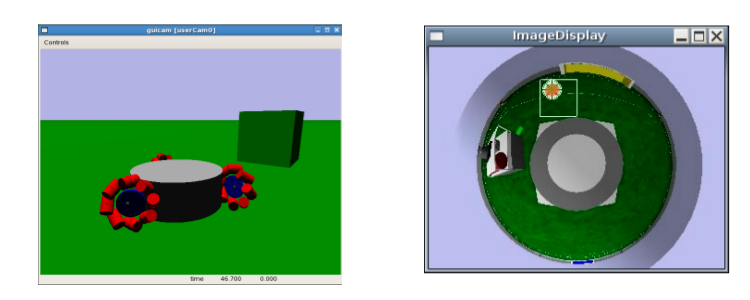
\includegraphics[scale=0.5]{pics/GazeboEquipment}
\label{Figure 2}
\caption{An omni-directional wheel prototype built in Gazebo (left) and the simulated picture taken of an omni-vision camera (right)~\cite{{MultiLevelAbstraction}}.}
\end{figure}
The omni-directional wheels of the Robotino work in the same way, but have a different design that needs to be modeled. The omni-vision camera mounted on the Robotino of Carologistics is very similar to the camera on the soccer-robots. The Gazebo-plugin for this camera might be a help for this thesis. The main point of~\cite{{MultiLevelAbstraction}} is the multi-level abstraction of the simulation. That means that the simulation is able to simulate with different levels of complexity. For example, the simulation can simulate on the physical level, where the robot software has to do movements and sensing as in the real world, and on a high logical level, where the robot moves exactly like intended and the simulation tells the robot exactly where it is located. These different abstraction levels are also important for the proposed thesis because they make the simulation more flexible and are well suited as milestones of the development of the simulation. \cite{{MultiLevelAbstraction}}~also shows that the speed of the simulation is an important aspect. If the simulation does not run fast enough to simulate in real-time, the behavior of the simulated robots may change because many processes running on the agent measure the time themselves. \cite{{MultiLevelAbstraction}}~dealt with this problem by changing the source code of the robot-software to use the simulation time instead of the system time. This is also possible in Fawkes because all plugins can use the time provided by Fawkes.\\
Another related work is~\cite{{SurveillanceSystem}}. It uses Gazebo and Player to simulate a surveillance system with Pioneer3AT robots. In this system several robots have to monitor an outdoor area and find possible intruders. Therefore, the robots have to spread over the area and coordinate their movements. The simulation was important for the development of the system because it could quickly simulate different areas and situations.\\
The 3D-Soccer-Simulation League in the RoboCup uses SimSpark as simulator\footnote{\url{http://www.robocupgermanopen.de/sites/default/files/rules_GO_2013_3Dsim.pdf}}. In this league two teams of eleven NAO robots each play in the simulation. The competition and comparison between the different approaches of multi-agent strategies make this league interesting for the thesis. There are some works such as~\cite{{SoccerChampion}} which show the capability of the simulator to simulate complex movements and agent architectures.
\subsection{Multi-Robot Coordination Strategies}
An example of complex multi-robot coordination strategies, that the simulation should be able to test, is \textit{Murdoch}. However, the thesis covers simpler approaches at the first place. Murdoch was presented by~\cite{DissMurdoch} and is an auction-based task allocation strategy. It solves a special instance of the \textit{Optimal Assignment Problem}. The Optimal Assignment Problem is to assign $n$ weighted jobs to $m$ workers with nonnegative skill ratings $h_{i,j}$ for each worker-job combination. Each worker is capable of doing one job at a time and each job can only be done by one worker. The task is to find the assignment which optimizes the performance, taking into account the weights of the jobs and the skill ratings of the workers to the jobs. The Murdoch method was especially developed 
for multi-robot scenarios. Therefore, it was designed to be able to handle robot failure and communication message loss. If a robot discovers a new task, it becomes an auctioneer and publishes a broadcast message to inform other robots about the task. All robots that are capable of doing the task calculate a metric of how well they probably will perform on the task. This metric is sent as a bid to the auctioneer. Finally the auctioneer decides after a predefined time interval which robot gets the task and informs this robot. After the allocation, the auctioneer observes the progress of the task and starts a new auction if the robot assigned in the first place fails. This method is decentralized but not optimal. However, \cite{DissMurdoch}~showed that the method performs well in different multi-agent tasks.\\

\section{Details of Work}
\subsection{Goals}
This section presents the goals of the thesis and how they will be reached in detail:
\begin{itemize}
\item \textbf{Simulation environment for LLSF:} Developing a simulation of LLSF means in detail to create a realistic environment in the simulation similar to Figure 1. The communication between Fawkes and Gazebo will be realized by using Google's Protocol Buffers\footnote{\url{http://code.google.com/p/protobuf/}}. Google Protocol Buffers is commonly known as Protobuf. It provides a flexible and easy to use data exchange format. It is possible to define messages in $.proto$ files. These files can be compiled to generate code files in different languages, such as C++ or Java. This simplifies using Protobuf in the own code. The main reason for choosing Protobuf for communication is that it is used in the Gazebo API and in~\cite{{KlingenDA}}.
\end{itemize}
On the one hand the movement orders from Fawkes will be executed in Gazebo and on the other hand the Gazebo plugins will simulate the sensing and will send the data to Fawkes. These two sides of the simulation will be developed in different detail-levels.
\begin{itemize}
\item \textbf{High level simulation:} In the high level simulation, Gazebo tells Fawkes ground truth about the simulated Robotinos. This includes the exact position, gyro-values and state of the objects which should be found by vision. All movement commands are executed exactly as intended. This level of simulation allows debugging and comparison of multi-robot strategies on a high logical level. All perception and motion control problems are left out.
\item \textbf{Low level simulation:} In the low level simulation, Fawkes receives only raw laser-data with and Gaussian error and captured images. The movements are realized by using the physics engine and the rotation of the wheels. This allows a more realistic simulation and testing of the whole system. For example, collisions between robots can be simulated. Furthermore it is possible to run isolated tests of perception and motion-control components.
\item \textbf{Simulation of multiple and communicating agents:} An important task of the thesis is the simulation of multiple robots controlled by separately running Fawkes instances in the same Gazebo environment at the same time. A global administrator plugin or a mechanism to map the Fawkes instances to the simulated Robotino plugins is necessary. The communication between the Fawkes instances does not have to be simulated because the local network is available. On the other hand, it is useful to simulate network latency and failure because there often are WiFi problems at RoboCup competitions. Therefore the communication can also be simulated on different levels.\\
\item \textbf{Expandability of the simulation:} Achieving abstraction in the implementation is important, so changes of LLSF or the Robotino can easily be integrated and other developments beside LLSF can benefit from this thesis. Two examples for such changes are that Festo recently presented a new Robotino version and the Technical Committee of LLSF decided to merge the two separate fields to one big field. The approach, to tackle expandability, is to build abstract sensors and actuators for the simulation for Fawkes and Gazebo. The present and future components can then specify the abstract ones. The abstract components encapsulate the communication between Fawkes and Gazebo as well as other functionality that is not domain specific. Furthermore the robot and field model of the simulation have to be exchangeable. All this is done as a second step to achieve a working simulation more quickly and to benefit from the knowledge gained in the first run.
\item \textbf{Multi-level abstraction:} The multi-level abstraction similar to~\cite{{MultiLevelAbstraction}} follows after the implementation of the high and low level simulation. Afterwards, it should be possible to choose the detail-level of the simulation.
\item \textbf{Simulation of LLSF challenges:} Another goal is to simulate the technical challenges of LLSF. For example there is a \textit{Whack-A-Mole} challenge. A robot has to reach machines, which give light signals, as fast as possible. This can be simulated by changing the behavior of the machines in the simulation environment.
\item \textbf{Comparison of different multi-robot strategies:} The comparison of different multi-robot strategies to solve the LLSF task is a long term goal of the Carologistics team. An efficient strategy has to be found and optimized to get good results in LLSF. The thesis compares strategies to prepare further work and to show the capabilities of the simulator. Strategies that can be compared are the current role-based approach, Murdoch and a job market system. The job market system decides which tasks have to be done and assigns tasks to idle robots. Therefore the robots have to inform the job market about their world belief and the success or failure of their tasks.
\item \textbf{Qualitative and quantitative evaluation of simulation:} The evaluation-goals are shown in detail in the next section.
\end{itemize}

\subsection{Implementation Structure}
As said before, the work will structurally consist of plugins for Gazebo and plugins for Fawkes. Similar to~\cite{{KlingenDA}} the Gazebo-plugins will be a robot-control plugin and an object-creator plugin. In addition, robot-sensor plugins and an LLSF-control plugin are needed. The LLSF-control plugin receives game-state inforamtion via Protobuf from the refbox and sends orders back when a puck was placed under a machine in the simulation. On the other side, there will be Fawkes plugins  for the sensors and for the Robotino to control the movements.\\
The implementation should be extendable to be able to easily implement future changes of robot hardware and LLSF game logic.

\subsection{Schedule}
\begin{table}
\centering
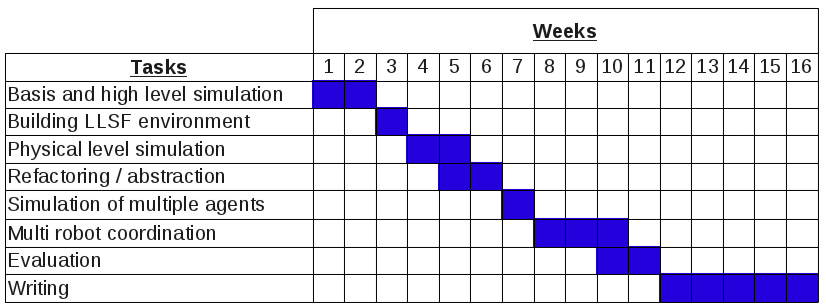
\includegraphics[scale=0.45]{pics/Schedule.png}
\label{Table 1}
\caption{Time-schedule}
\end{table}

The time-schedule of the thesis is shown in Table 1. There is enough buffer-time to handle unexpected problems or to go further, implement more features and reach higher goals. There are two weeks buffer on the practical level and two weeks after the writing. These buffers are this large due to the difficulty of estimating the needed time for the defined goals.

\subsection{Evaluation}
This section covers the evaluation of the proposed thesis. On the one hand a qualitative analysis should show if and how well the simulation generally works. On the other hand the thesis will give a quantitative analysis of the performance and scalability of the simulation.\\
The qualitative evaluation analyzes the functionality of the simulation and the realized features. It will evaluate which components and problem scenarios can be well simulated and where there are difficulties in the other problem scenarios. The aim of the evaluation is to compare the robot's behavior in the simulation to that in reality. To do this, it is necessary to look at the difference in the sensor data first because this may be the main cause for different behavior. Furthermore, the difference of multi-robot behavior needs to be analyzed. This will be more challenging because of the greater complexity.\\
In the quantitative evaluation the speed of the simulation is important because a difference between real-time and simulation-time can also cause differences in the behavior. The network latency can be a cause for difference in the coordination between the robots. Another part of the quantitative evaluation is to measure the CPU and memory usage. Because the thesis is about a multi-robot simulation, the scalability of the simulation has to be measured, too. This means to measure the simulation speed, CPU and memory usage in relation to the number of robots simulated.

\section{Conclusion}
The thesis proposed here will develop a multi-robot simulation environment for LLSF with Fawkes and Gazebo. It is the basis for efficient and quality-assured work of current and future developments. The simulation environment will concentrate on the LLSF league, which provides a testbed for research on logistic robots. The proposal showed that Gazebo is well suited as simulator for this thesis and future work. A part of the thesis will be built on previous work by~\cite{{KlingenDA}} and~\cite{{MultiLevelAbstraction}}. The proposal also defined the main~goals. The evaluation will look at qualitative and quantitative aspects to ensure the quality and performance of the simulation.\\
An important advantage of the thesis is the support future work. Although the simulation is primarily made for LLSF, it is also an important step for other developments because Gazebo can simulate almost every robot and other simulations can base on this thesis. Furthermore the proposal showed that a multi-robot simulator is a key to an effective development of multi-robot coordination.


\bibliographystyle{plain}
\bibliography{references}

\end{document}
